\documentclass{article}

\usepackage{color}
\usepackage{graphicx}
\usepackage{amsmath}
\usepackage{geometry}
\usepackage{setspace}
\usepackage{listings}
\usepackage{xcolor}
\lstset{
    columns=fixed,       
    numbers=left,                                       
    frame=none,                                          
    backgroundcolor=\color[RGB]{245,245,244},            
    keywordstyle=\color[RGB]{40,40,255},                 
    numberstyle=\footnotesize\color{darkgray},           
    commentstyle=\it\color[RGB]{0,96,96},                
    stringstyle=\rmfamily\slshape\color[RGB]{128,0,0},   
    showstringspaces=false,                              
    language=c++,                                        
}
\geometry{left=2.54cm,right=2.54cm,top=2.54cm,bottom=2.54cm}
\begin{document}
\begin{spacing}{2.0}
\vspace*{0.25cm}

\hrulefill

\thispagestyle{empty}

\begin{center}
\begin{large}
\sc{UM--SJTU Joint Institute \vspace{0.3em} \\ Introduction to Operating Systems \\(VE482)}
\end{large}

\hrulefill

\vspace*{5cm}
\begin{Large}
\sc{{Homework 2}}
\end{Large}

\vspace{2em}

\end{center}


\vfill

\begin{table}[h!]
\flushleft
\begin{tabular}{lll}
Name: Ji Xingyou \hspace*{2em}&
ID: 515370910197\hspace*{2em}
\\

Date: 28 September 2017

\end{tabular}
\end{table}

\hfill

\newpage
\noindent\textbf{Ex.1} -- \textit{Multiprogramming}\\
\begin{enumerate}
\item What is the probability for n processes to be waiting at the same time, then express the CPU utilisation as a function of n?\\
\textbf{probability:}
$p^n$

\textbf{CPU utilisation:}
$1-p^n$
\item Sketch the curve representing the CPU utilisation as a function of the number of processes for the following values of p: 25\%, 60\% and 90\%.\\
\begin{figure}[!h]
	\begin{center}
	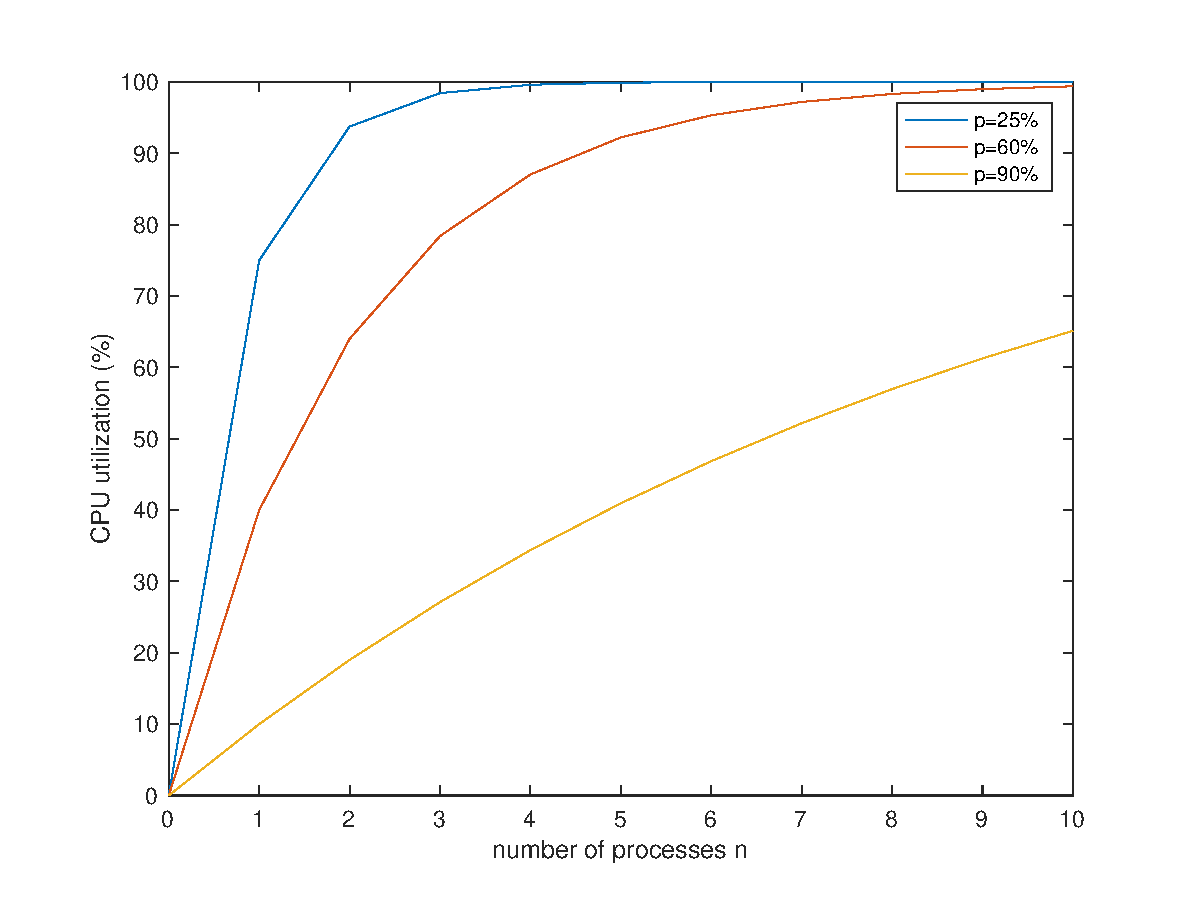
\includegraphics[scale=0.9]{multiprogramming.eps}
	\caption{CPU utilization vs n}
	\end{center}
\end{figure}\\
Below is the Matlab code.
\begin{lstlisting}[language=Matlab]
clear all;clc;
syms n CPU_utilization1;
n=0:1:10;
p1=0.25;
p2=0.6;
p3=0.9;
CPU_utilization1=(1-p1.^n)*100;
plot(n,CPU_utilization1);
hold on;
CPU_utilization2=(1-p2.^n)*100;
plot(n,CPU_utilization2);
hold on;
CPU_utilization3=(1-p3.^n)*100;
plot(n,CPU_utilization3);
xlabel('number of processes n');
ylabel('CPU utilization (%)');
legend('p=25%','p=60%','p=90%');
\end{lstlisting}
\item A certain old computer has 256 MB of RAM, once loaded a light operating system uses 96 MB of RAM. Several programs are launched each of them using 48 MB.
\begin{itemize}
    \item How many processes can be store simultaneously in memory?\\
    $n=[\frac{256-96}{48}]=[\frac{160}{48}]=3$
    \item Assuming an average of 90\% I/O waiting time what is the CPU utilisation?\\
    $CPU utilizaiton=1-p^n=1-90\%^3=27.1\%$
    \item What is the effect of adding 256 MB, 512 MB and 1024 MB of RAM. Argue on which amount would be the most beneficial and would be worth the investment.\\
    \textbf{256 MB:}\\
    $n=3+\frac{256}{48}=3+5=8$\\
    $CPU utilization=1-p^n=1-90\%^8=56.95\%$\\
    $\Delta=56.95-27.1=29.85\%$\\
    \textbf{512 MB:}\\
    $n=3+\frac{512}{48}=3+10=13$\\
    $CPU utilization=1-p^n=1-90\%^13=74.58\%$\\
    $\Delta=74.58-56.95=17.63\%$\\
    \textbf{1024 MB:}\\
    $n=3+\frac{1024}{48}=3+21=24$\\
    $CPU utilization=1-p^n=1-90\%^{24}=92.02\%$\\
    $\Delta=92.02-74.58=17.44\%$\\
    Therefore, adding 256 MB is most beneficial.
\end{itemize}
\end{enumerate}
\noindent\textbf{Ex.2} -- \textit{Keymap in Minix 3}\\
First, in the dmp.c file, add SF7.
\begin{lstlisting}[language=c++]
struct hook_entry {
    int key;
    void (*function)(void);
    char *name;
} hooks[] = {
    { F1,   proctab_dmp, "Kernel process table" },
    { F3,   image_dmp, "System image" },
    { F4,   privileges_dmp, "Process privileges" },
    { F5,   monparams_dmp, "Boot monitor parameters" },
    { F6,   irqtab_dmp, "IRQ hooks and policies" },
    { F7,   kmessages_dmp, "Kernel messages" },
    { F8,   vm_dmp, "VM status and process maps" },
    { F10,  kenv_dmp, "Kernel parameters" },
    { SF1,  mproc_dmp, "Process manager process table" },
    { SF2,  sigaction_dmp, "Signals" },
    { SF3,  fproc_dmp, "Filesystem process table" },
    { SF4,  dtab_dmp, "Device/Driver mapping" },
    { SF5,  mapping_dmp, "Print key mappings" },
    { SF6,  rproc_dmp, "Reincarnation server process table" },
    { SF7,  proc_num_dmp,"Currently running processes number"}
    { SF8,  data_store_dmp, "Data store contents" },
    { SF9,  procstack_dmp, "Processes with stack traces!" },
};
\end{lstlisting}
Then, in the proto.h, add the declaration of the proc$\_$num$\_$dmp function.
\begin{lstlisting}[language=c++]
/* dmp_kernel.c */
void proc_num_dmp(void);
void proctab_dmp(void);
void procstack_dmp(void);
void privileges_dmp(void);
void image_dmp(void);
void irqtab_dmp(void);
void kmessages_dmp(void);
void monparams_dmp(void);
void kenv_dmp(void);
\end{lstlisting}
Finally, in the dmp$\_$kernel.c, add the implementation of the proc$\_$num$\_$dmp function.
\begin{lstlisting}[language=c++]
void proc_num_dmp(void)
{
    register struct proc *rp;
    int r;
    if((r=sys_getproctab(proc))!=OK)
    {
        printf("IS: warning: couldn't get copy of process table: %d\n", r);
        return;
    }
    
    int num=0;
    for(rp=BEG_PROC_ADDR;rp<END_PROC_ADDR;rp++)
    {
        if(isemptyp(rp))
        {
            continue;
        }
        num++;
    }
    printf("Currently running processes number is:  %d\n", num);
}
\end{lstlisting}
\end{spacing}
\end{document}